\documentclass[12pt, letterpaper]{article}
\usepackage[english]{babel}
\usepackage{graphicx}
\usepackage{float}
\usepackage{hyperref}

\title{DAT510 - Assignment 2}
\author{Fr\o ydis J\o rgensen}

\begin{document}
\begin{titlepage}
\maketitle
\end{titlepage}

\begin{abstract}
A one-paragraph summary of the entire assignment - your choices of cryptographic primitives and their parameters,
procedure, test results, and analysis. 
\end{abstract}

\section*{Introduction}
A description of the scientific background for your project, including previous work that your project builds on.
(Remember to cite your sources!) The final sentence (analogous to the thesis statement in a term paper) is the
objective of your experiment. 

\section*{Design and Implementation}
I have created both a digital signature scenario in the main with a predefined message where we can validate the signature on the message and two applications where Alice and Bob can send messages to each other with a signature and validate that the messages are correct. Both the main and the applications uses the same methods and I will therefore first explain all the methods before I go into the applications. \\

When implementing RSA, I think the most crucial thing is to find some good keys. We need two random large primes, \textbf{p} and \textbf{q}. By multiplying \textbf{p} and \textbf{q} we get \textbf{n}. The keys are generated as shown in Figure \ref{fig:generatePrimes}. To decide \textbf{p} and \textbf{q} I use a package called Crypto and uses their method \textit{getPrime}, and to get a random primes I also uses Crypto's function \textit{get\_random\_bytes}. Although the chances for p and q to be the same is very small, we should make sure that's not the case. I take in the bit length as an input to the function. There are major runtime differences that depend on the bit length, but I will get back to that.

\begin{figure}[H]
  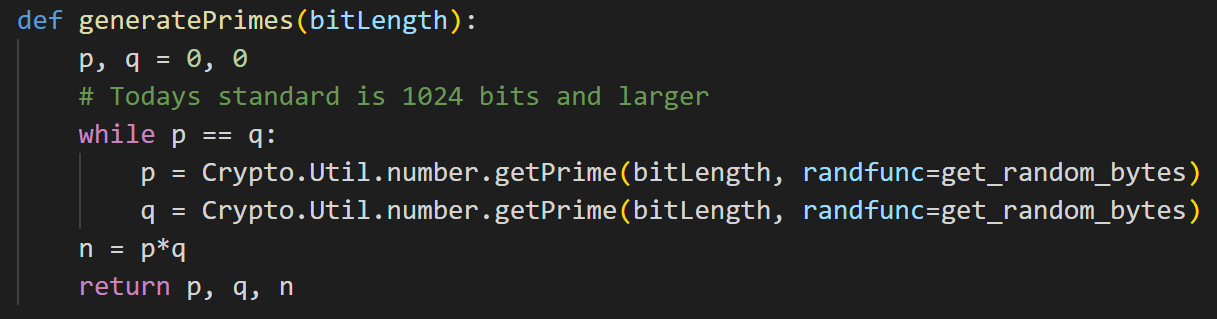
\includegraphics[width=\linewidth]{code_snippets/getPrimes.PNG}
  \caption{Generates two large primes and multiplies them}
  \label{fig:generatePrimes}
\end{figure}

The next step is to find the totient of \textbf{n}, $\phi$ phi. As shown in Figure \ref{fig:totient} that's an easy calculation using \textbf{p} and \textbf{q}.

\begin{figure}[H]
  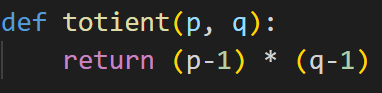
\includegraphics[width=150px]{code_snippets/totient.PNG}\centering
  \caption{Calculated the totient of n from p and q}
  \label{fig:totient}
\end{figure}

Together with \textbf{n} we have another public exponent \textbf{e}. This is a prime number that should be the greatest common divisor of 1 with $\phi(n)$. But it is often chosen to be the Fermat number 65537. That is the largest known prime in the form of $2^{2^{n}} + 1, (n=4)$. It is large enough to avoid attacks and quick on binary calculations. But we should always check that e is not a factor of the totient $\phi$. If that is the case, we choose the next largest prime number, \cite{65537}. As shown in Figure \ref{fig:e} I use \textit{gcd} imported from the package math to calculate the greatest common divisor.

\begin{figure}[H]
  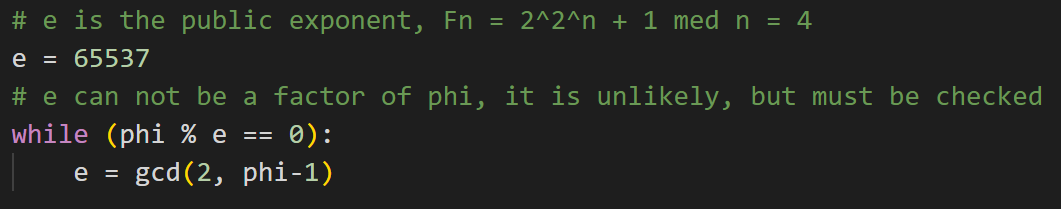
\includegraphics[width=\linewidth]{code_snippets/e.PNG}\centering
  \caption{e is F4, 65537, if it is a factor of the totient use the gcd}
  \label{fig:e}
\end{figure}

Using the public exponent \textbf{e} and $\phi$ we can create the private exponent \textbf{d}. The private exponent \textbf{d} is the inverse of the public exponent with respect to the totient $\phi$. To calculate the inverse you can use the \textit{Extended Euclidean Algorithm}. I have taken an implementation of that from geeksforgeeks, ref \cite{modinv}. This method works when \textbf{e} and $\phi$ is coprimes, which we already know they are. The function to find \textbf{d} is shown in Figure \ref{fig:modinv}

\begin{figure}[H]
  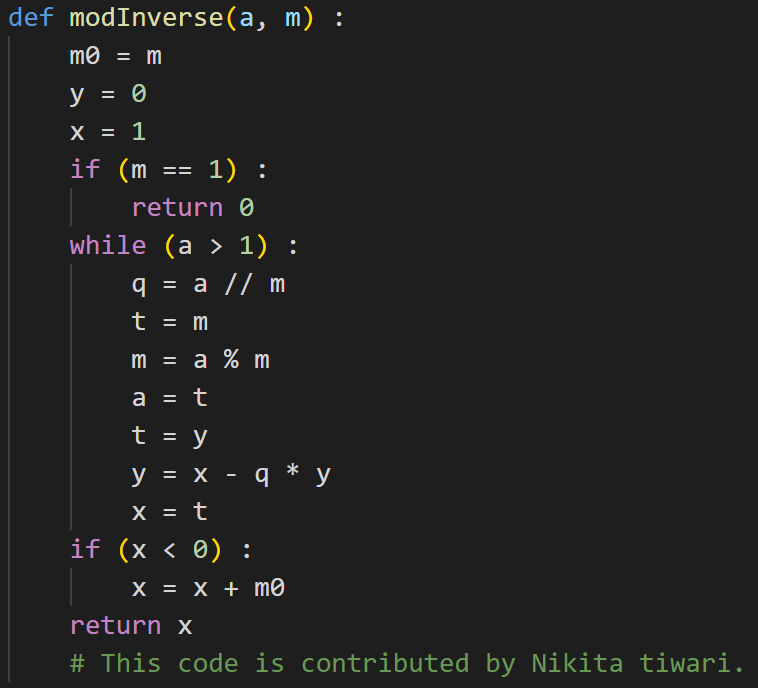
\includegraphics[width=250px]{code_snippets/modinv.PNG}\centering
  \caption{Finding the inverse. Function from GeeksforGeeks}
  \label{fig:modinv}
\end{figure}

Now that we have the public keypair of \textbf{e} and \textbf{n} and the private keypair of \textbf{d} and \textbf{n}, we can start creating the digital signature on the message. Before we can run the RSA encryption calculation to create the signature we have to hash the original data (the message). I have imported \textit{hashlib} and used SHA256 for hashing the message. So that means that no matter how long the message is, we will get a 256 bit block.
Using the hash we can now create the signature by using RSA's encryption function. We will use our private key to create the signature as shown here in the mathematical expression.
$$hash^{d}\ mod\ n$$
In the code, as shown in Figure \ref{fig:hash}, I use the function \textit{pow} which does the same as the mathematical expression. As you can also see in the figure is that I convert the hash into an integer, and throughout the program I only work with integers instead of bits.

\begin{figure}[H]
  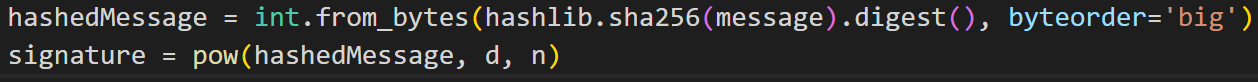
\includegraphics[width=\linewidth]{code_snippets/hash.PNG}\centering
  \caption{Hashing the message and create signature}
  \label{fig:hash}
\end{figure}

Now that we have the message and the digital signature we can send it and verify that the message is correct according to the signature and it have not been tampered by some man in the middle. To verify the signature we take the message and creates a hash using the same hashing method SHA256. This hash should match what we decrypt from the signature. To decrypt the signature we do the same mathematical operation as when it was created but instead of the message, we use the signature, and instead of the private key \textbf{d} we use the public key \textbf{e}. This works because both \textbf{e} and \textbf{n} is public keys. So in this case everyone can verify that the message was sent from f.ex Alice. Normally we would use some encryption on top of that, since the message now is sent in plaintext. As you can see in Figure \ref{fig:verify}, we check that the hash we got from the message is the same that we got after decrypting the signature. If they are the same, we have verified that the message from Alice is the same as at the point Alice signed it and sent it.

\begin{figure}[H]
  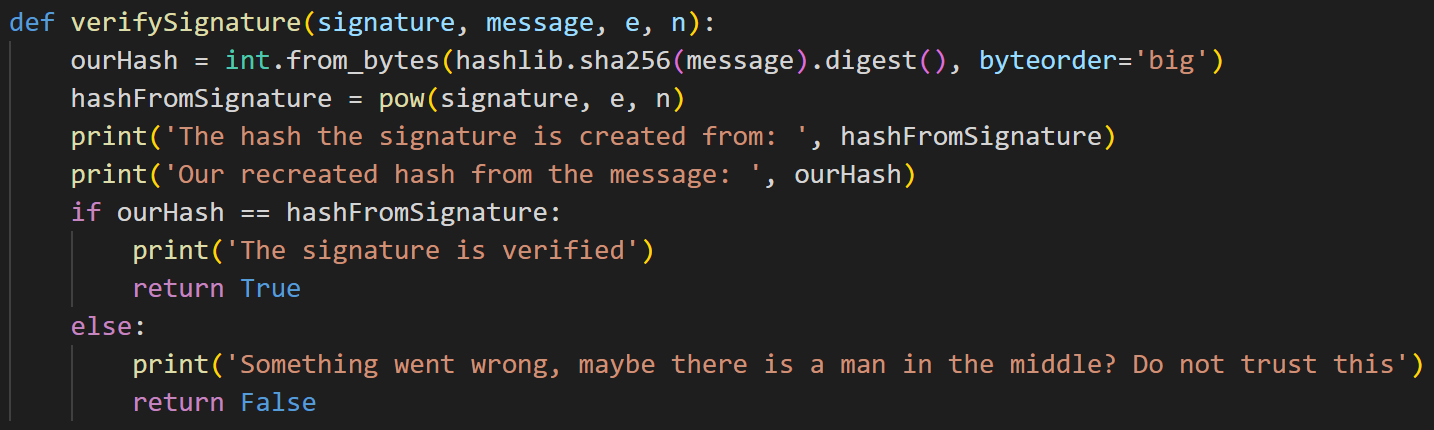
\includegraphics[width=\linewidth]{code_snippets/verify.PNG}\centering
  \caption{Verifying that the signature matches the message}
  \label{fig:verify}
\end{figure}

In the application we have two url's. The start url, where we can send a message and sign it. And /getMsg where we can see the message from the other part and see if the signature is correct. Opening the application will automatically run the generation of the public and private keys, in the same way as explained previously. \\

When a message is written and it's clicked send the signature will be created as shown in Figure \ref{fig:send}. The fetching point for people that want to receive the message is /sentMsg. And the message is sent as a dictionary including the message, the signature, \textbf{e} and \textbf{n}.
 
\begin{figure}[H]
  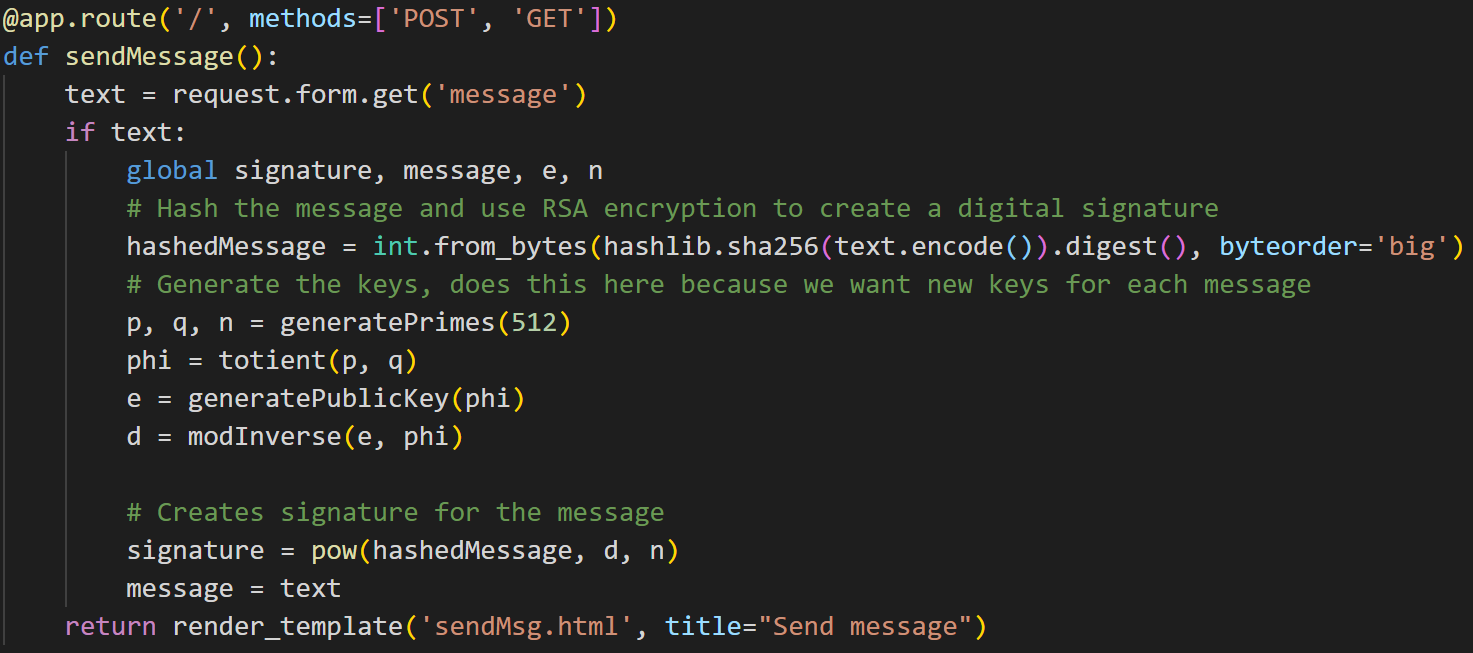
\includegraphics[width=\linewidth]{code_snippets/send.PNG}\centering
  \caption{Running a template with input field and submit button to send message with a signature}
  \label{fig:send}
\end{figure}

To fetch messages you go to /getMsg. If there is no message it will be displayed "There is no message". If there is a message we have to verify the signature. We use the \textit{verifySignature} method as shown in Figure \ref{fig:verify}. If the message and the signature corresponds the message will be shown with a note that the signature is correct. If the signature is wrong there is a warning that someone might have tampered the message.
 
\begin{figure}[H]
  \hspace*{-50px}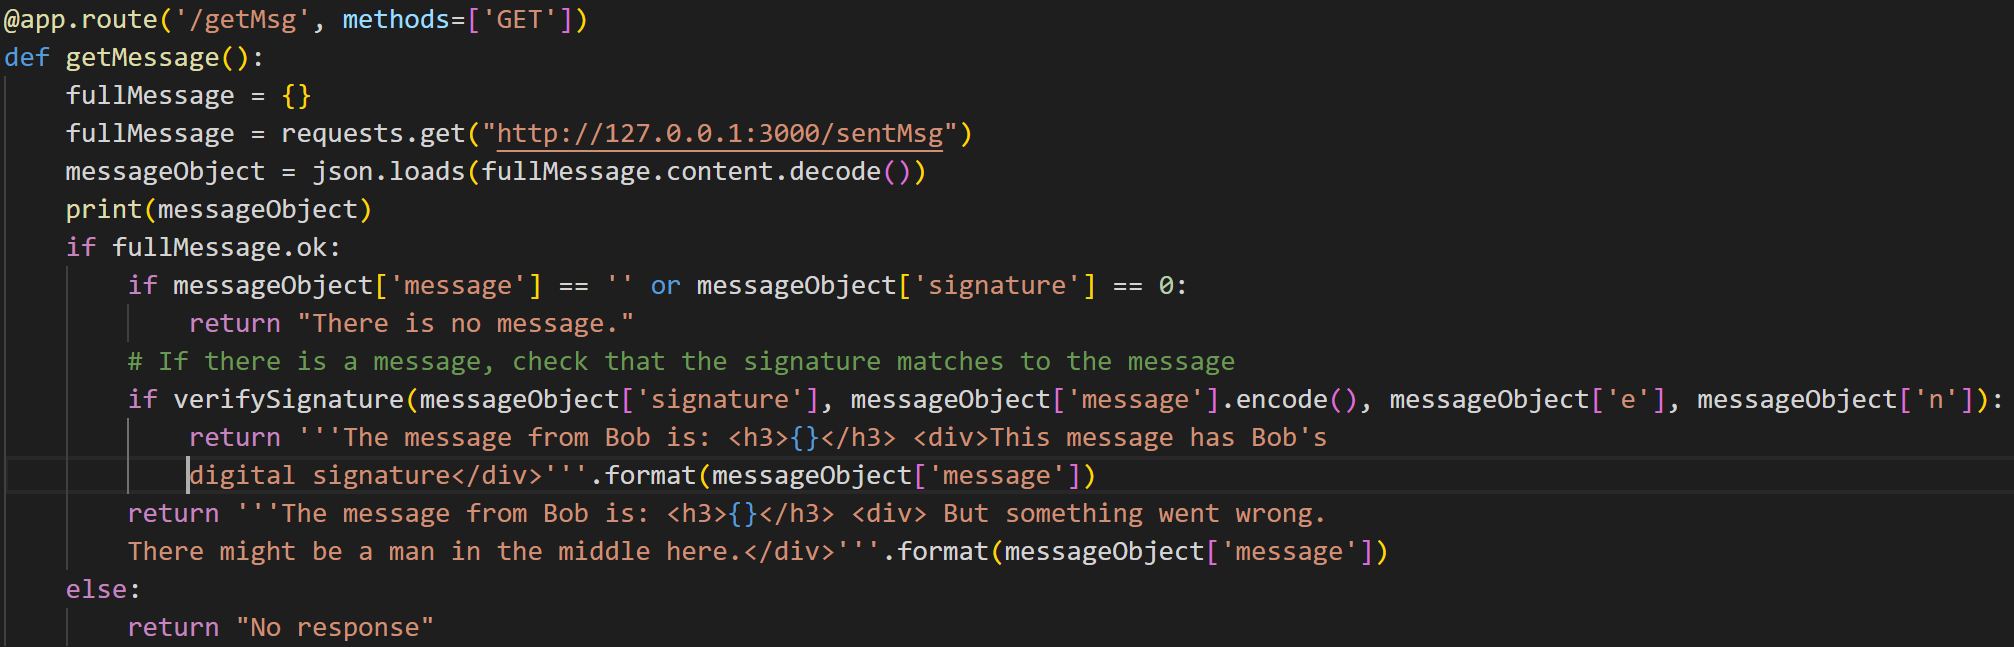
\includegraphics[width=500px]{code_snippets/get.PNG}\centering
  \caption{Fetching the message and verifying the signature}
  \label{fig:get}
\end{figure} 

The applications has a very very similar set up as in assignment 2, and one is run on port 3000 and one on port 5000. 

\section*{Test results}

Running the main applications will print out the information we get while doing a digital signature and verifying it. As you can see in Figure \ref{fig:print}, the first thing printed is the public and private keys. Then we can see the message sent from Alice to Bob and the signature sent with it. The recreated hash is created by Bob to see that it matches the hash we got by encrypting Alice's signature. And in this case they are the same and therefore the signature is verified.

\begin{figure}[H]
  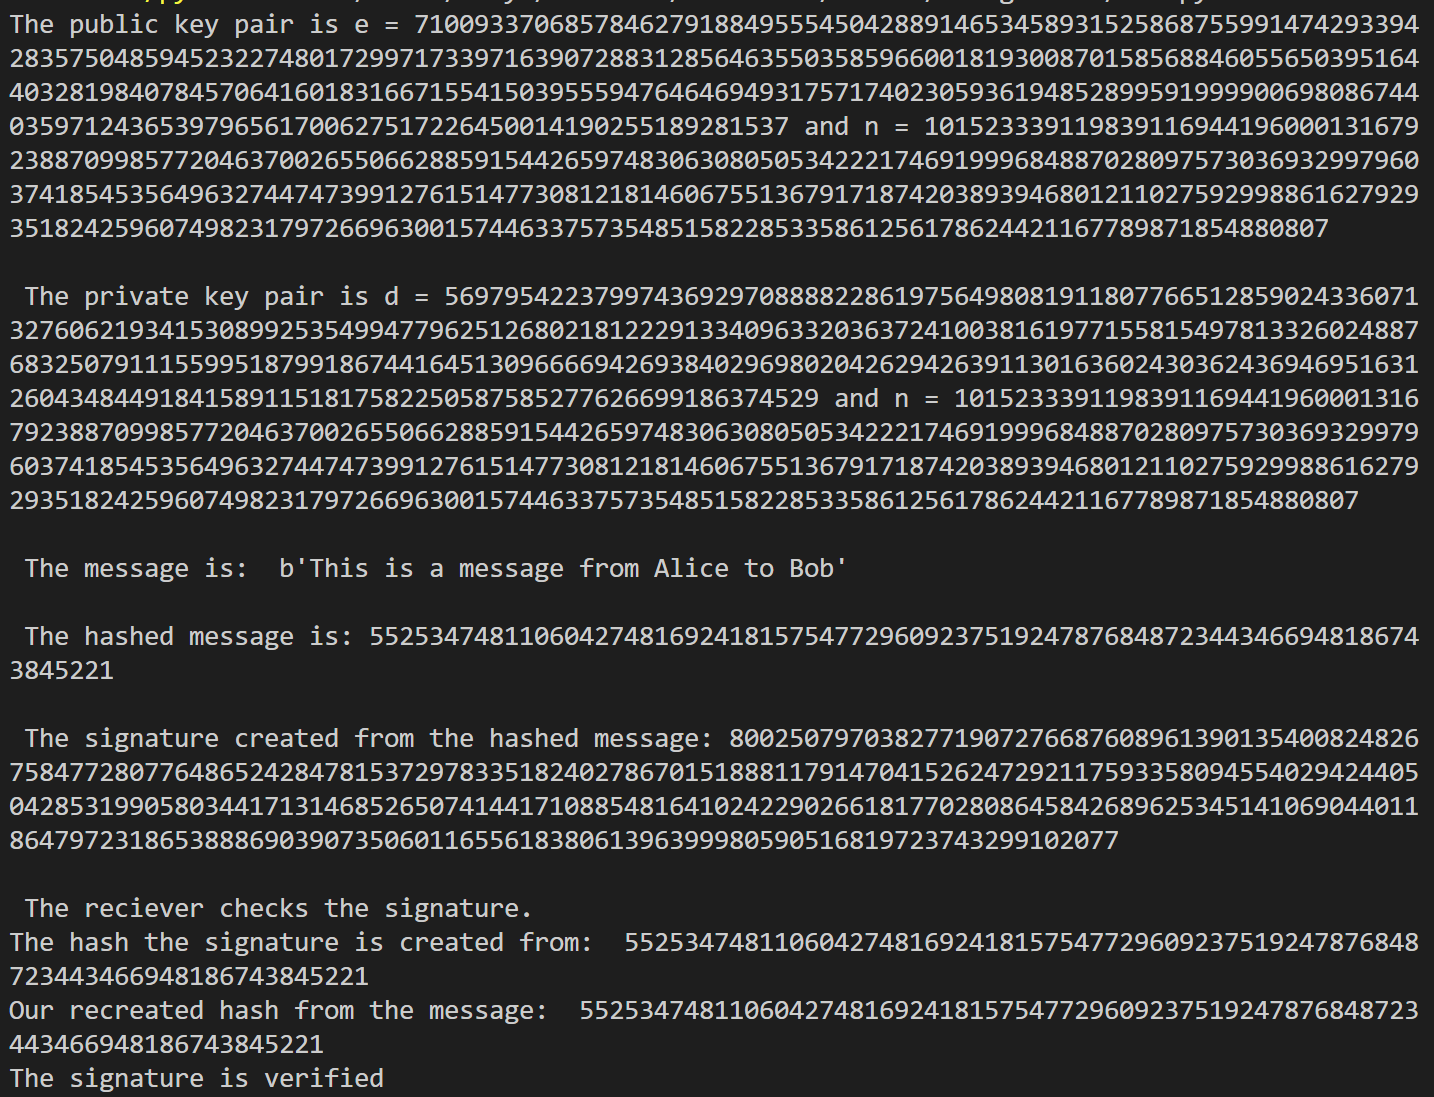
\includegraphics[width=\linewidth]{code_snippets/print.PNG}\centering
  \caption{The print statements from the RSA.py main}
  \label{fig:print}
\end{figure}

Using this on the two applications will look as shown in Figure \ref{fig:msg}, when the signature is verified. If the signature does not match the message, the note under the message will tell you that.

\begin{figure}[H]
  \hspace*{-50px}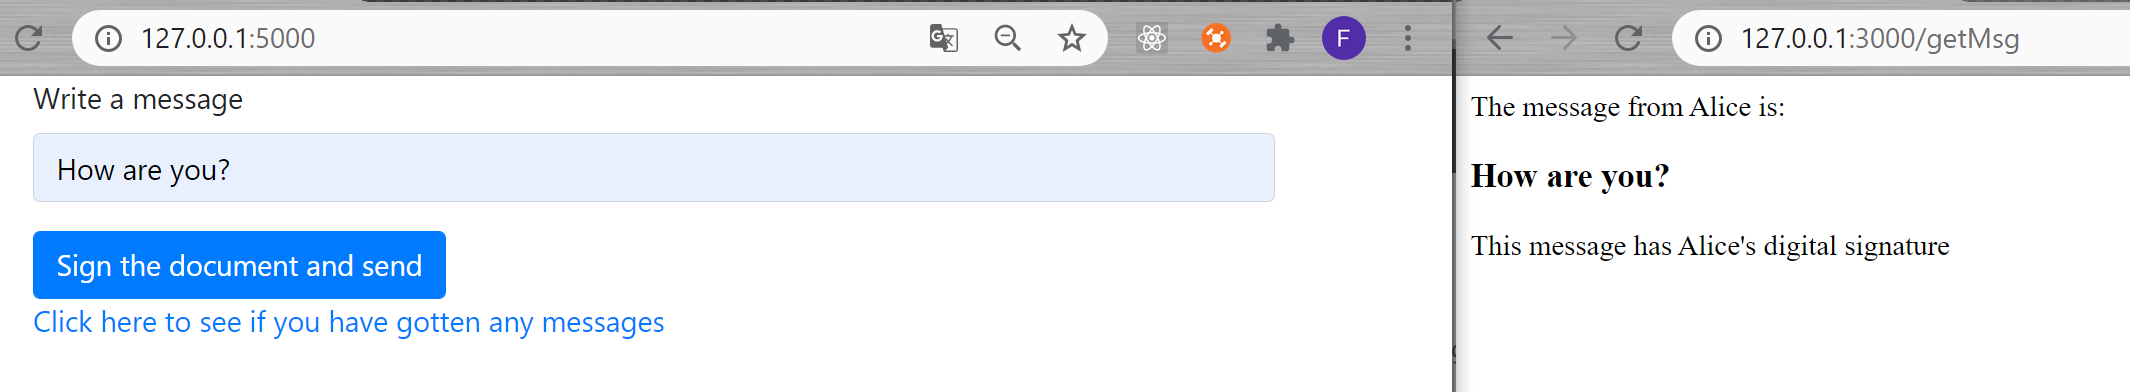
\includegraphics[width=500px]{code_snippets/msg.PNG}\centering
  \caption{Alice sends a message and sign it. Bob receives it and verifies the signature}
  \label{fig:msg}
\end{figure}

It seems like RSA usually uses key of 2048 bits. Creating and working with that big numbers goes slow in python and to beware of computational problems I have used the package \textit{timeit} to find out the different execution times depending on the bit length. You can see the result in the table here.

\begin{center}
\begin{tabular}{ |c|c|c| } 
 \hline
 Bit length & Execution time\\
 128 & 0.060 \\ 
 256 & 0.186 \\ 
 512 & 0.738 \\ 
 1024 & 4.894 \\ 
 2048 & 35.01 \\
 \hline
\end{tabular}
\end{center}

As you can see in the table, the execution time increases exponentially as we increases the bit length.

\section*{Discussion}
Your analysis of what your testing results mean, and your analysis.

I could have, and was thinking about splitting up the message, to get a lower runtime, but did not see that as a must in this case, since the messages was not that big anyway. I tried sending a string with 5000 characters, and it was slower, but nothing crucial.

\section*{Conclusion}
A short paragraph that restates the objective from your introduction and relates it to your results and discussion, and
describes any future improvements that you would recommend. Works Cited A bibliography of all of the sources
you got information from in your report. 


\begin{thebibliography}{10} 
\bibitem{65537} 65,537,  \emph{Wikipedia - The number 65537},
\url{https://en.wikipedia.org/wiki/65,537}.
\bibitem{modinv} GeeksforGeeks,  \emph{Modular inverse},
\url{https://www.geeksforgeeks.org/multiplicative-inverse-under-modulo-m/}.
\end{thebibliography}



\end{document}